% Optical micrographs obtained from the Cone~5 On-Heating 2375\textdegree{}F (\gls{zdt}) sample are presented in Figure~\ref{fig:c5-oh-2375} and show the region adjacent to the fracture surface.  It is apparent from Figure~\ref{subfig:c5-oh-2375-50X} that the crack paths follow the interdendritic boundaries and that the greatest extent of crack opening along the boundaries generally occurs perpendicular to the hot ductility test tensile loading direction (also visible in Figure~\ref{subfig:c5-oh-2375-200X}).  A region of the Cone~5 On-Heating 2375\textdegree{}F (\gls{zdt}) sample which was remote from the fracture location (not subjected to the simulated thermal cycle) is shown in Figure~\ref{fig:c5-oh-2375-remote}.  Comparing Figure~\ref{subfig:c5-oh-2375-500X} and Figure~\ref{subfig:c5-oh-2375-remote-500x}, it is apparent that the extent of intradendritic precipitates is reduced in the vicinity of the fracture surface.


% \begin{figure}
% \centering
% \subfloat[50X]{\label{subfig:c5-oh-2375-50X}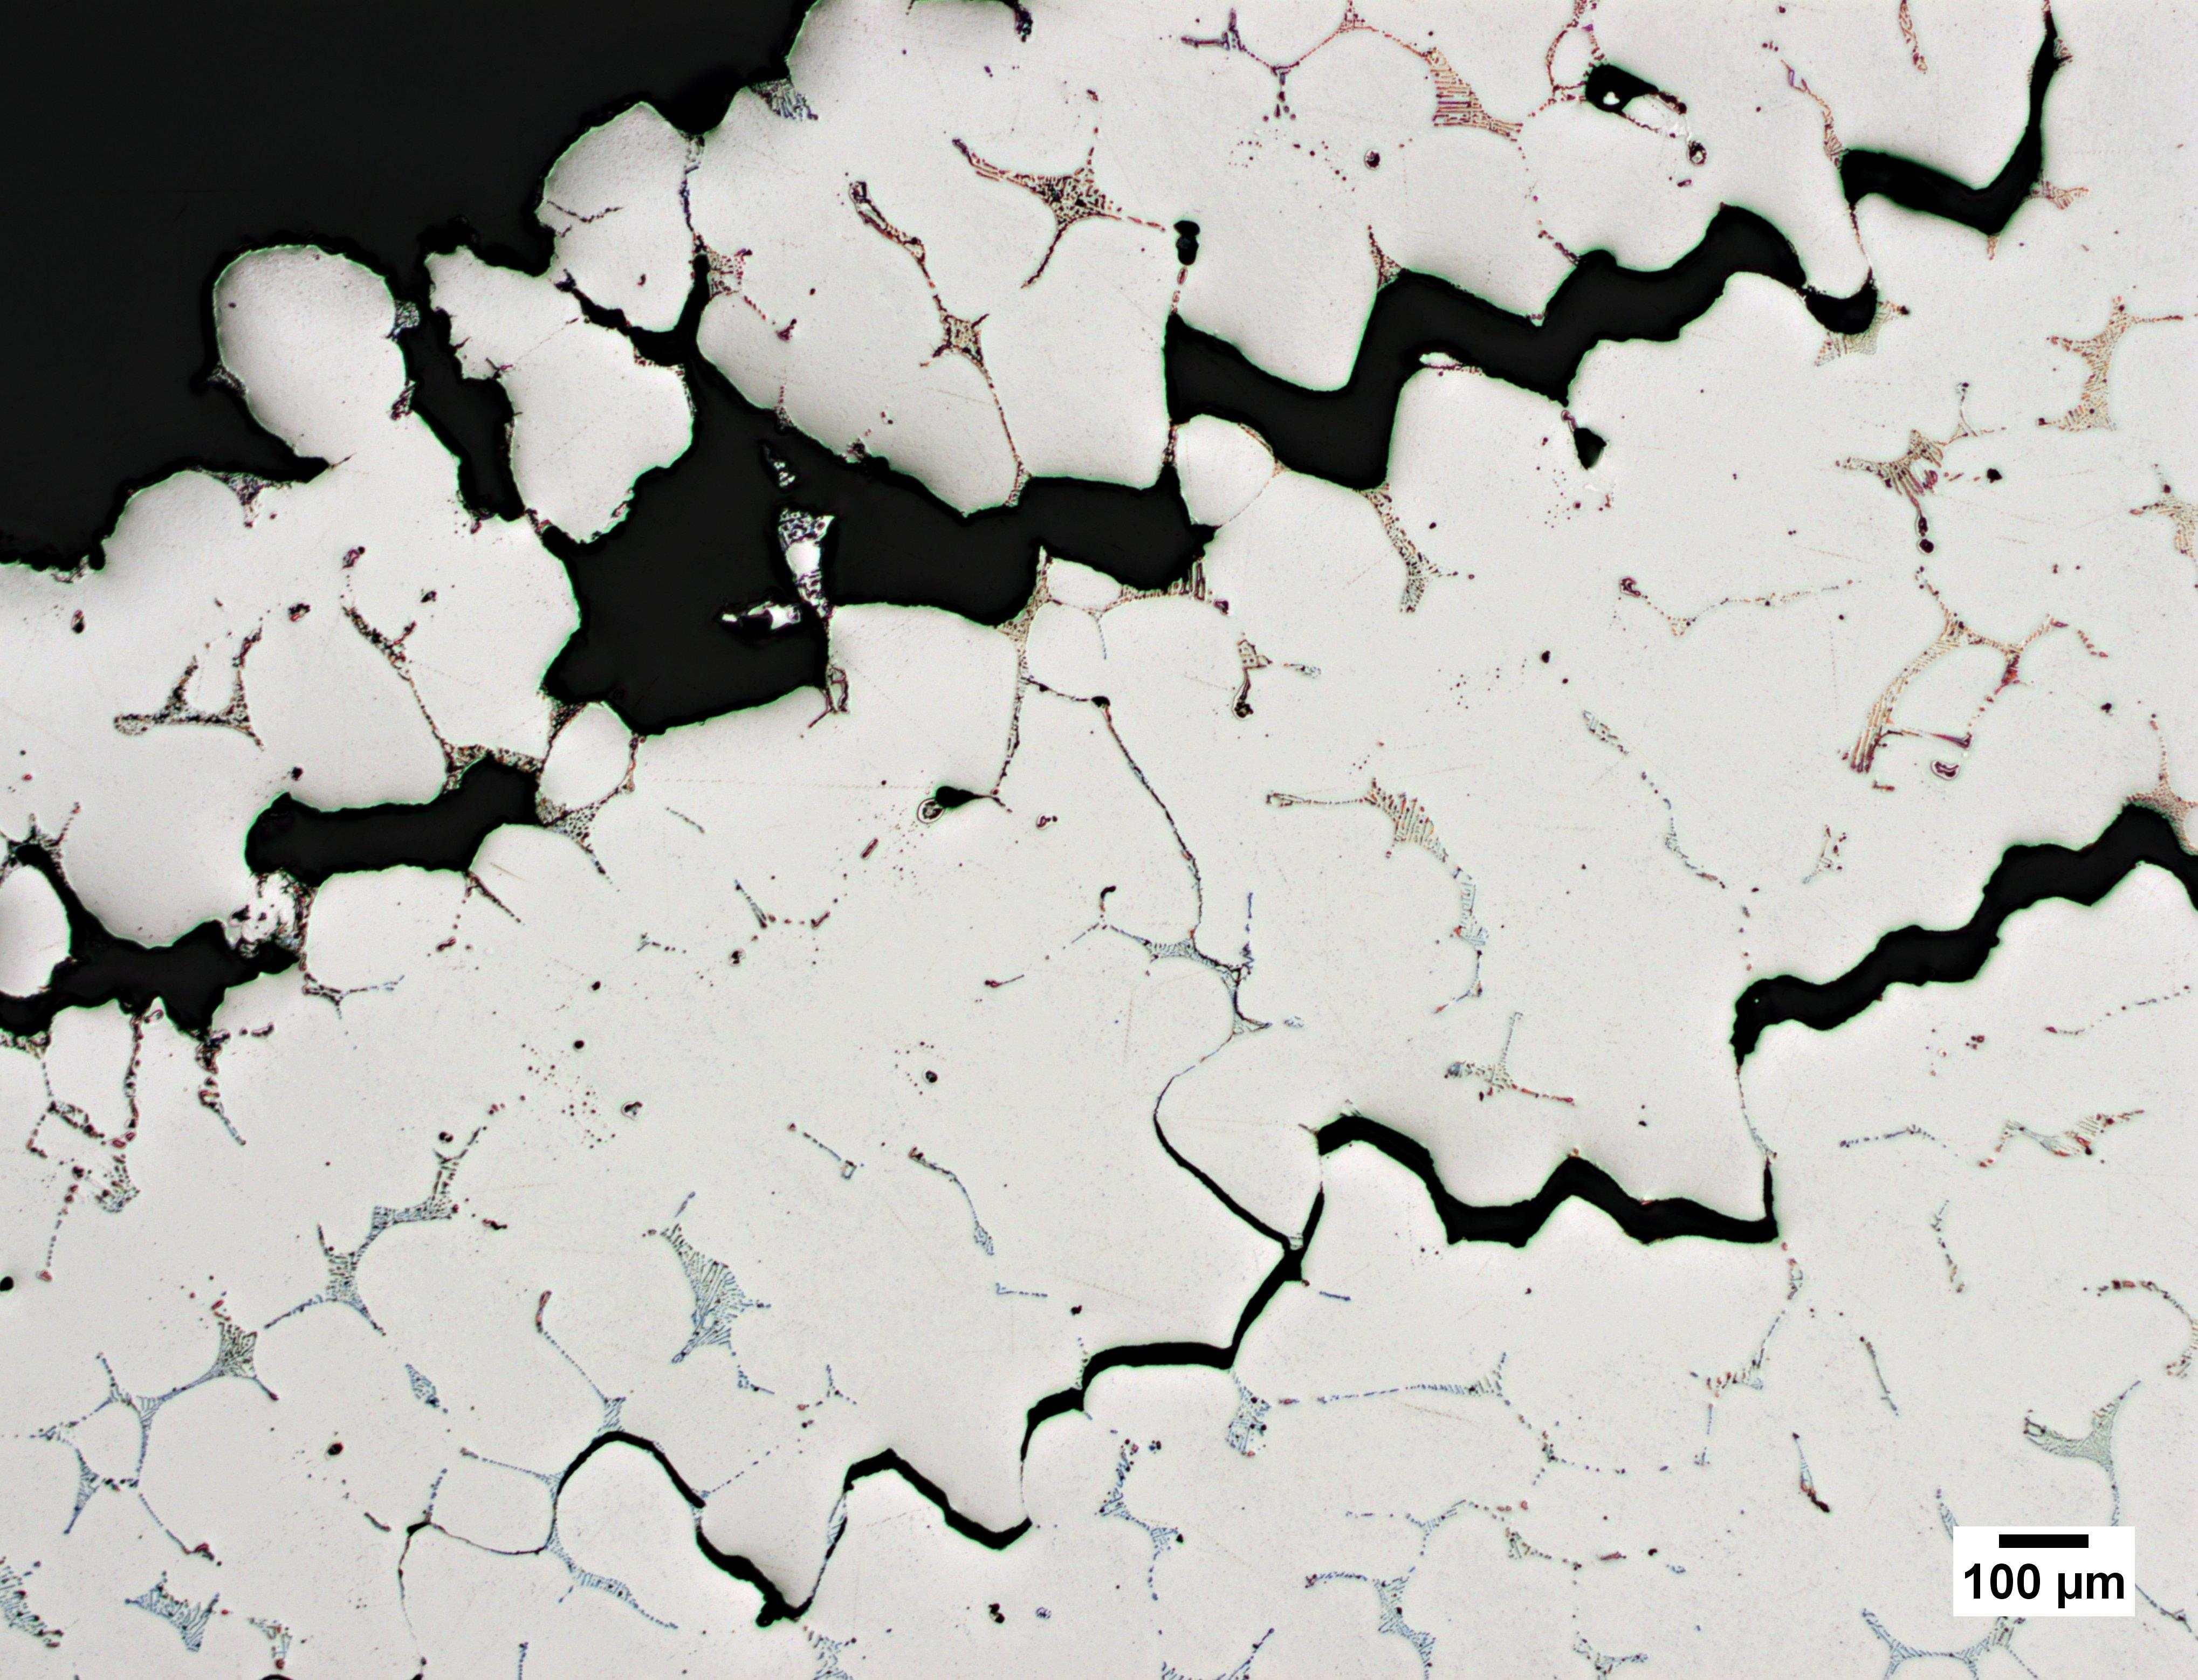
\includegraphics[width=4.7in]{figures/metallography/c5-oh-2375-50x}}\\
% \subfloat[200X]{\label{subfig:c5-oh-2375-200X}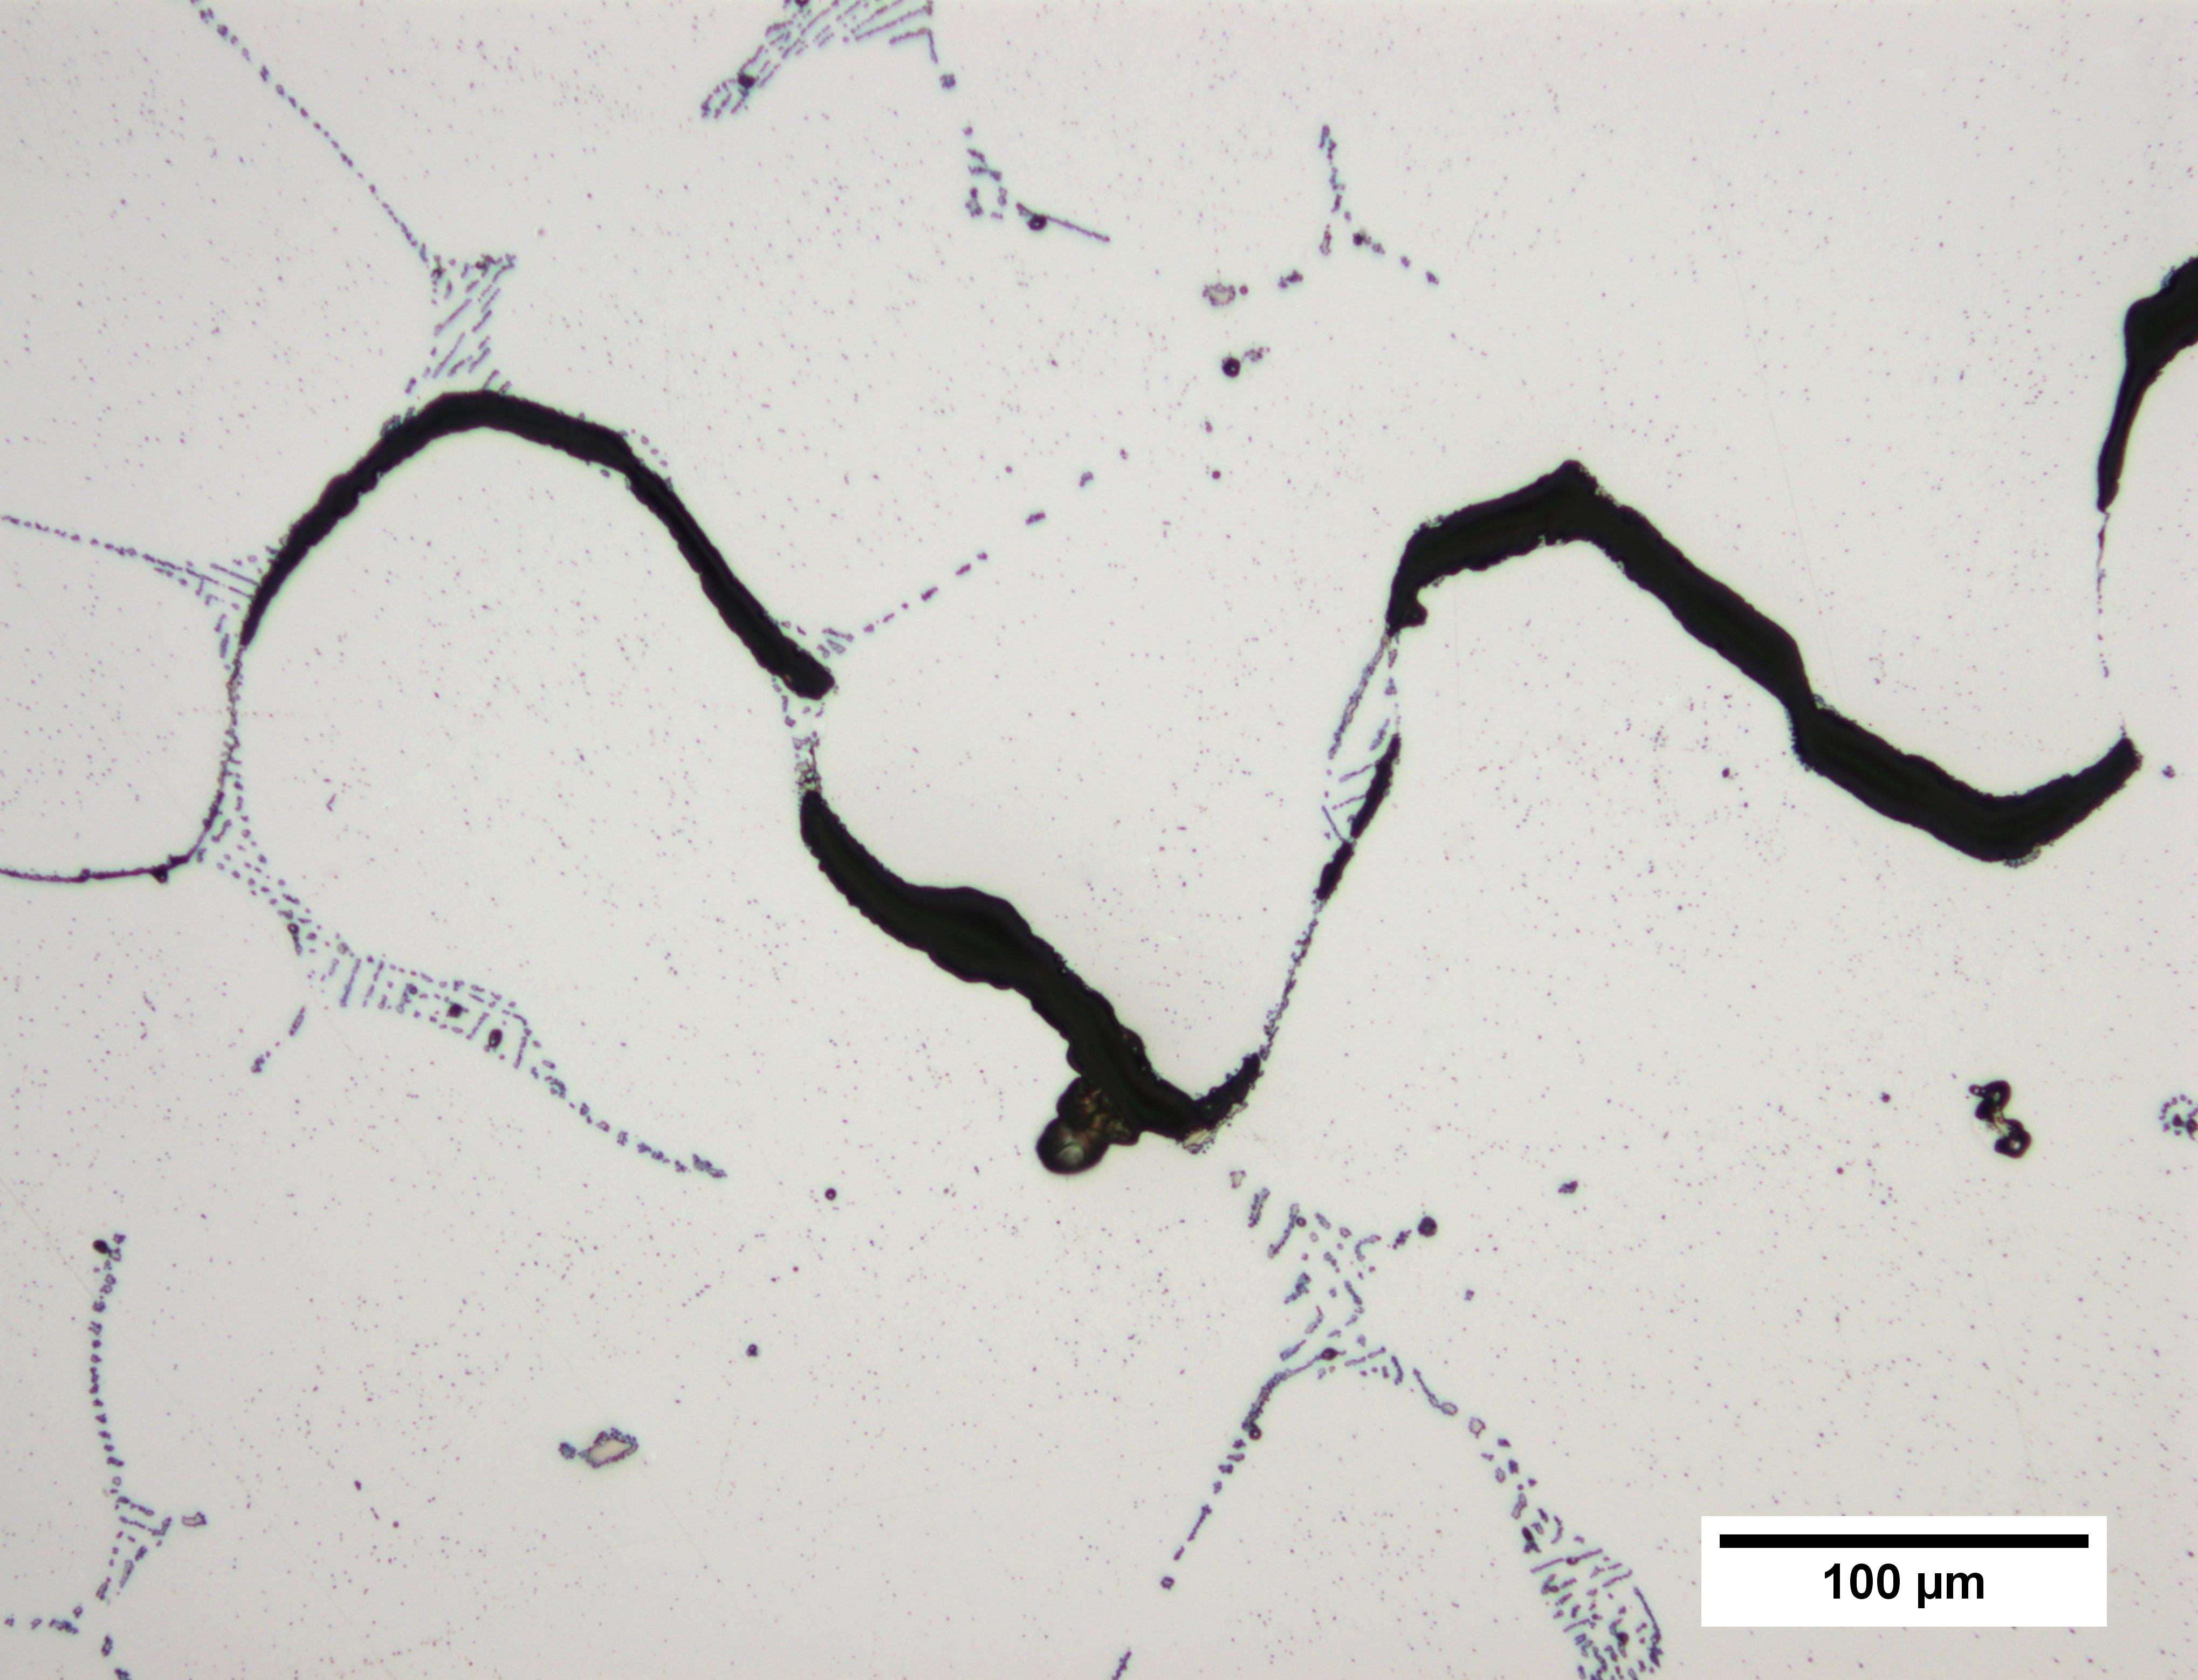
\includegraphics[width=4.7in]{figures/metallography/c5-oh-2375-200x}}

% \caption[Optical Micrographs Showing the Fracture Path as Revealed in a Longitudinal Section Through the Cone~5 2375\textdegree{}F On-Heating Hot Ductility Sample.]{Optical Micrographs Showing the Fracture Path as Revealed in a Longitudinal Section Through the Cone~5 2375\textdegree{}F On-Heating (\gls{zdt}) Hot Ductility Sample, at (A) 50X (B) 200X, (C) 500X and (D) 1000X.  Etch: electrolytic 10\% oxalic acid.}
% \label{fig:c5-oh-2375}
% \end{figure}


% \begin{figure}
% \ContinuedFloat
% \centering
% \subfloat[500X]{\label{subfig:c5-oh-2375-500X}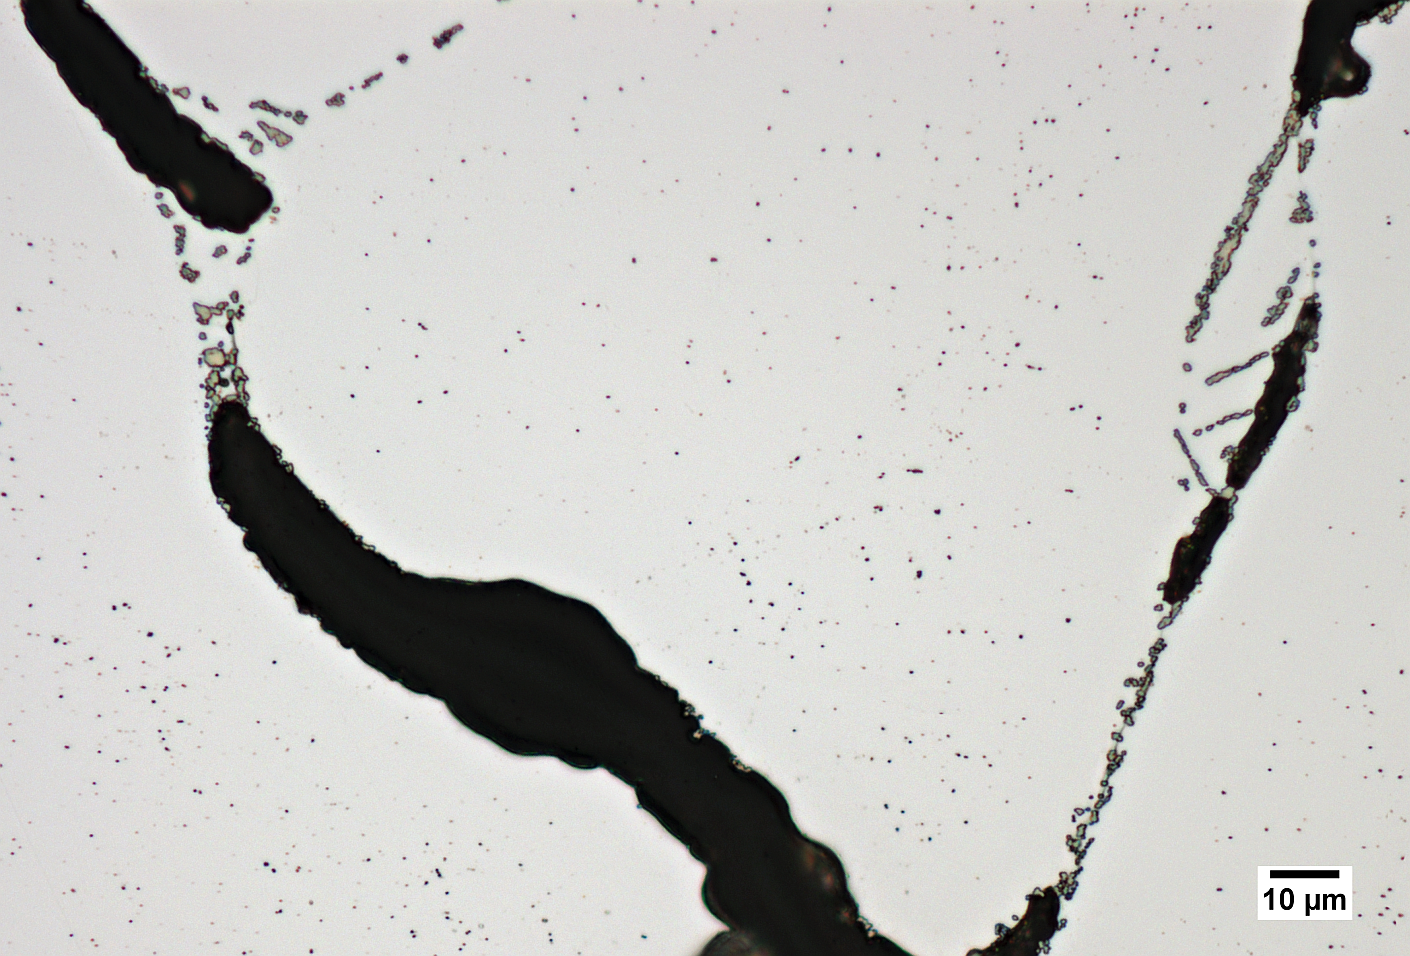
\includegraphics[width=4.7in]{figures/metallography/c5-oh-2375-500x}}

% \subfloat[1000X]{\label{subfig:c5-oh-2375-1000X}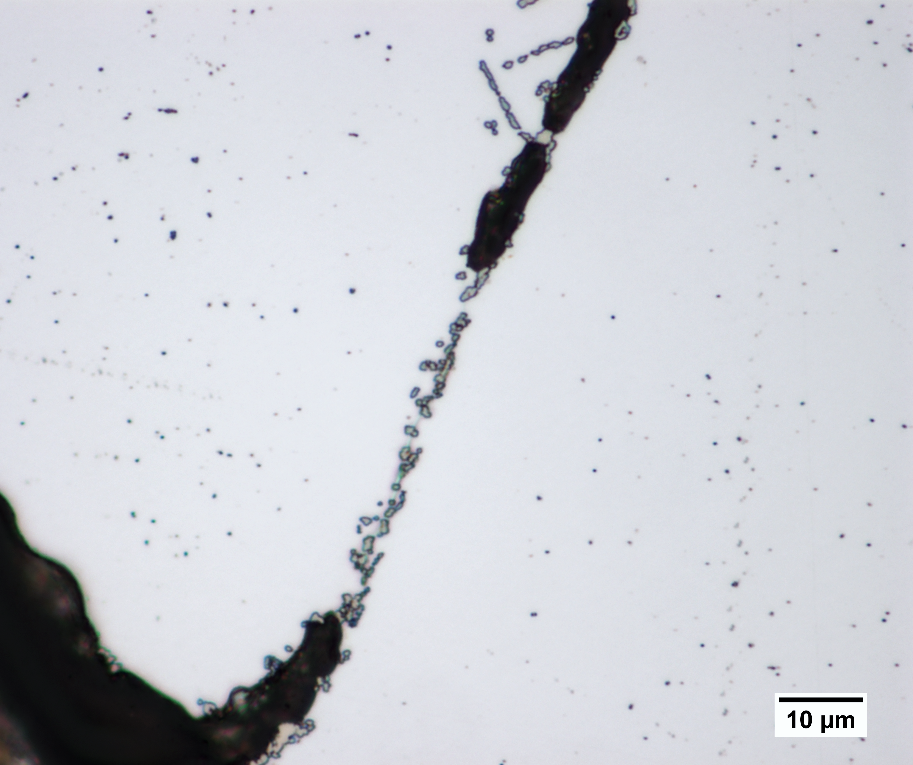
\includegraphics[width=4.7in]{figures/metallography/c5-oh-2375-1kx}}
% \caption[Optical Micrographs Showing the Fracture Path as Revealed in a Longitudinal Section Through the Cone~5 2375\textdegree{}F On-Heating Hot Ductility Sample.]{Optical Micrographs Showing the Fracture Path as Revealed in a Longitudinal Section Through the Cone~5 2375\textdegree{}F On-Heating (\gls{zdt}) Hot Ductility Sample, at (A) 50X (B) 200X, (C) 500X and (D) 1000X.  Etch: electrolytic 10\% oxalic acid.}

% \end{figure}


% \begin{figure}
% \centering
% \subfloat[200X]{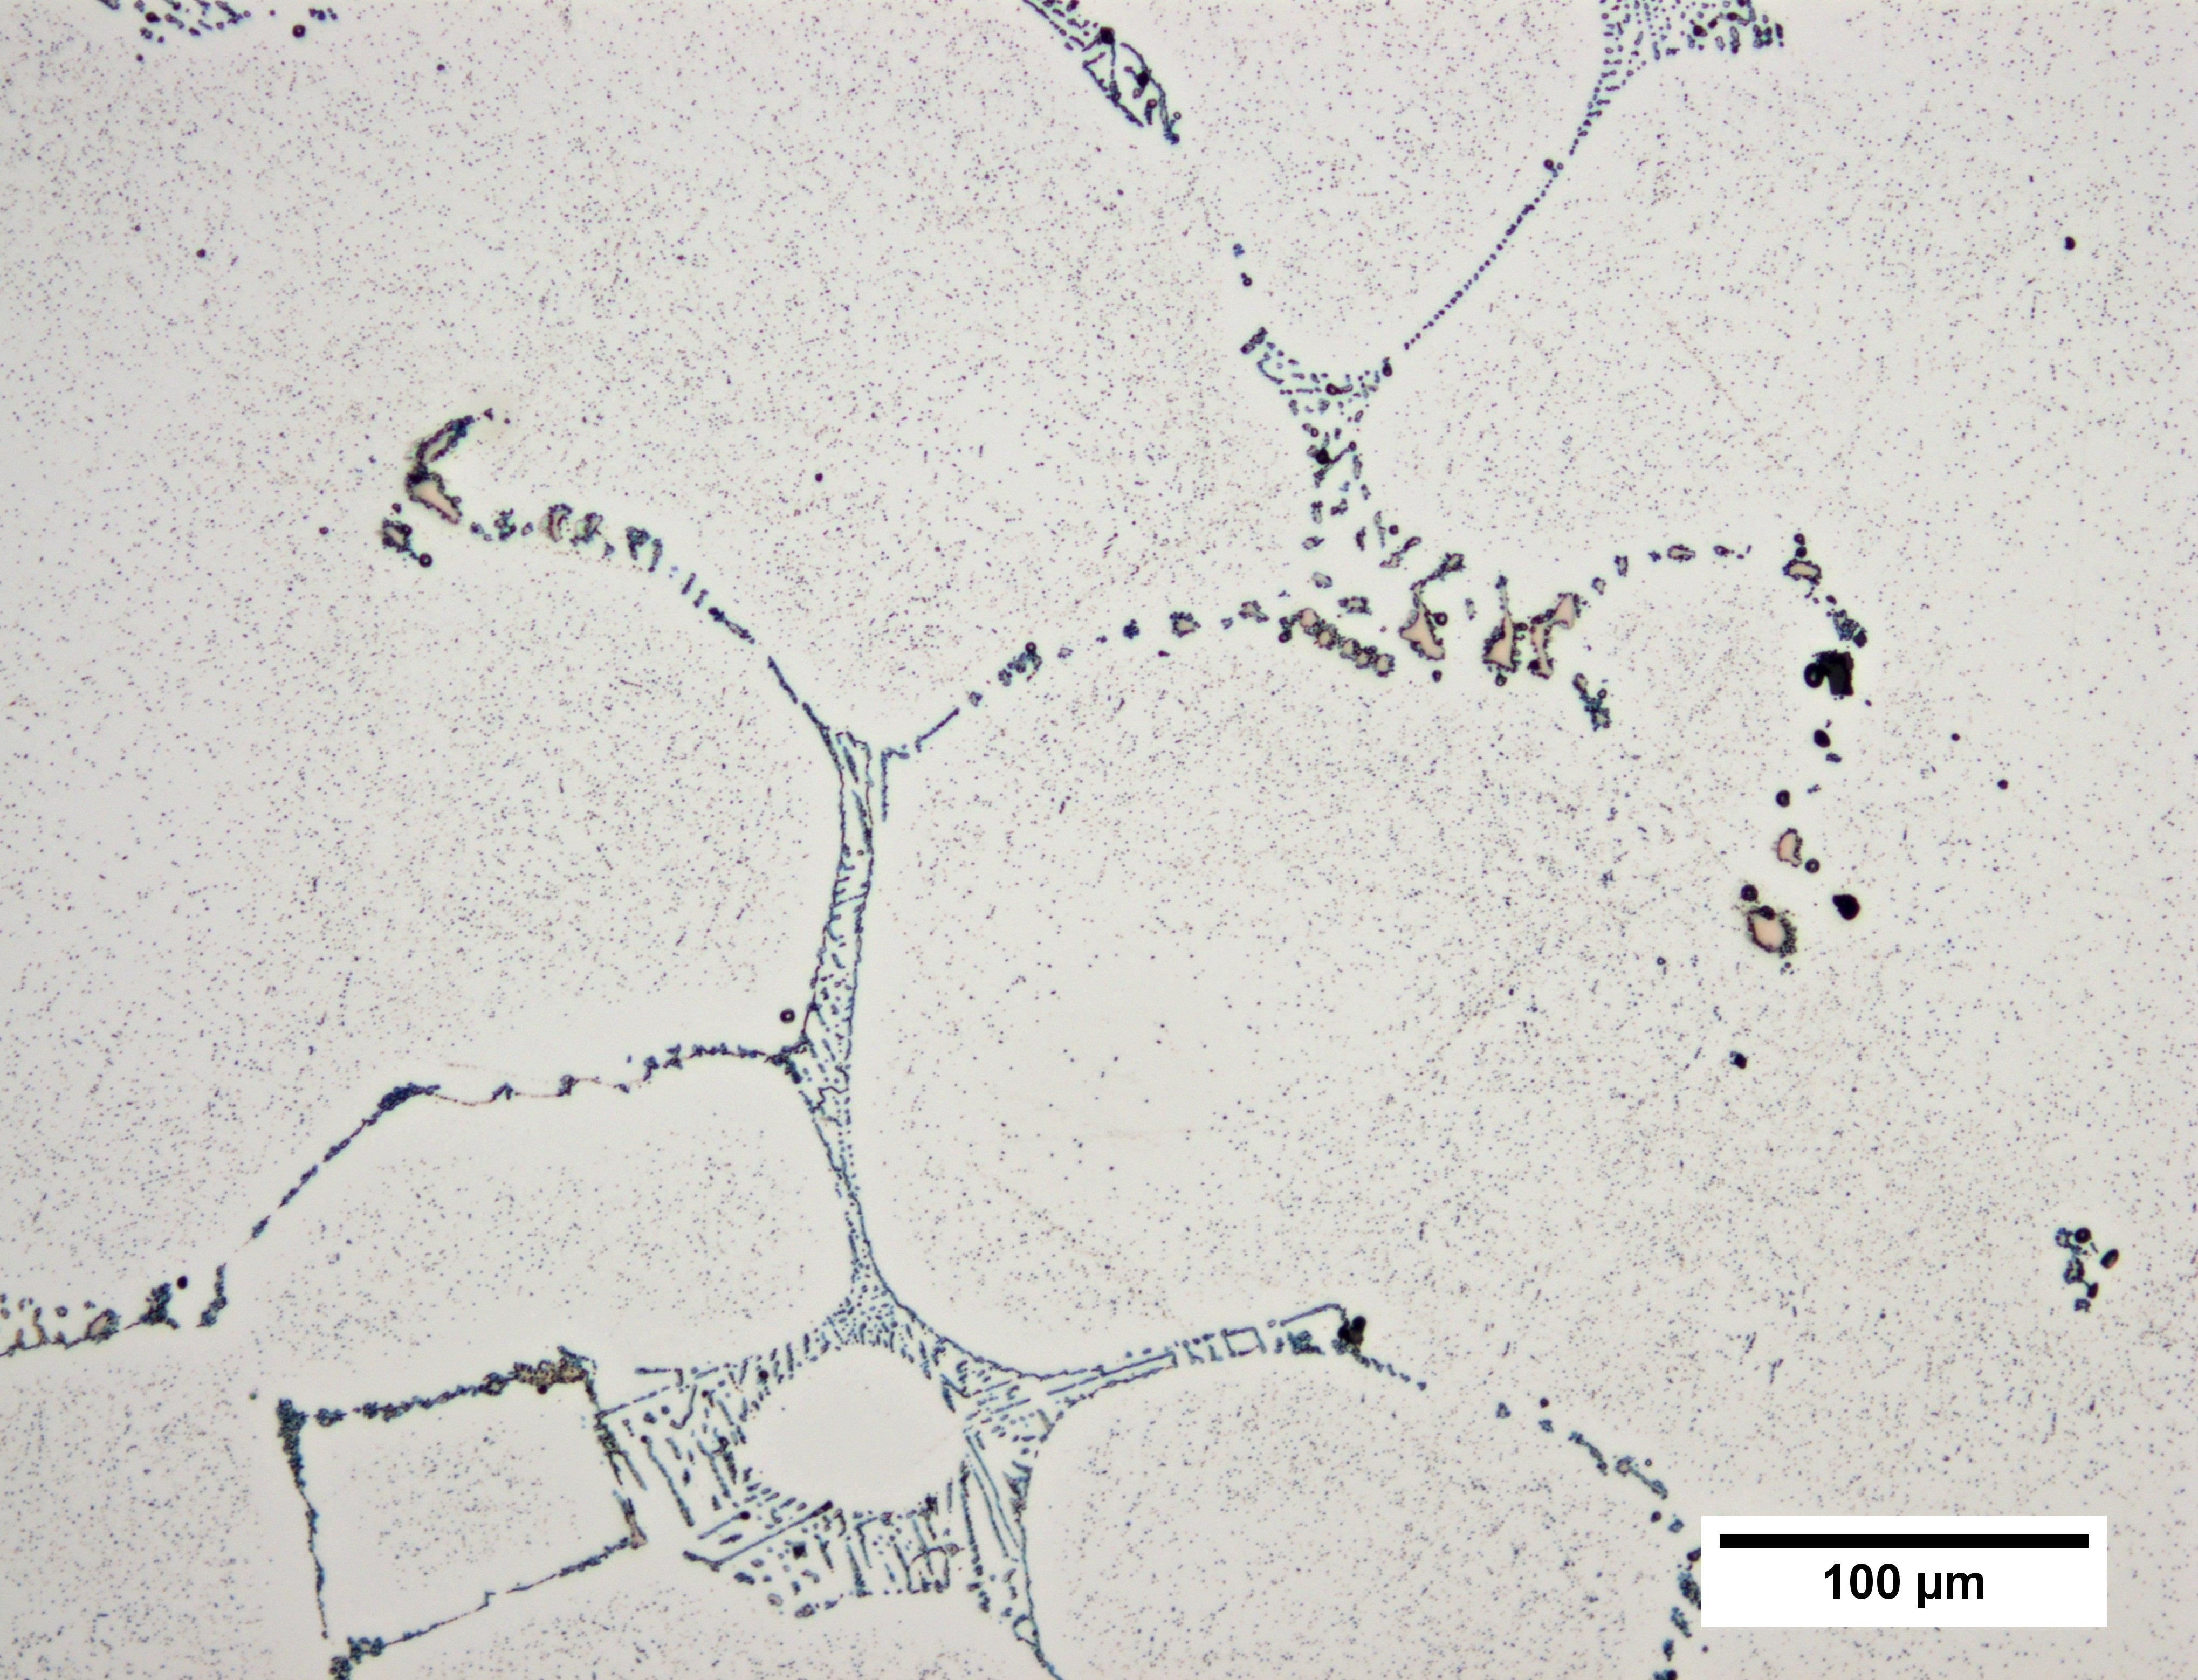
\includegraphics[width=4.7in]{figures/metallography/c5-oh-2375-remote-200x}}

% \subfloat[500X]{\label{subfig:c5-oh-2375-remote-500x}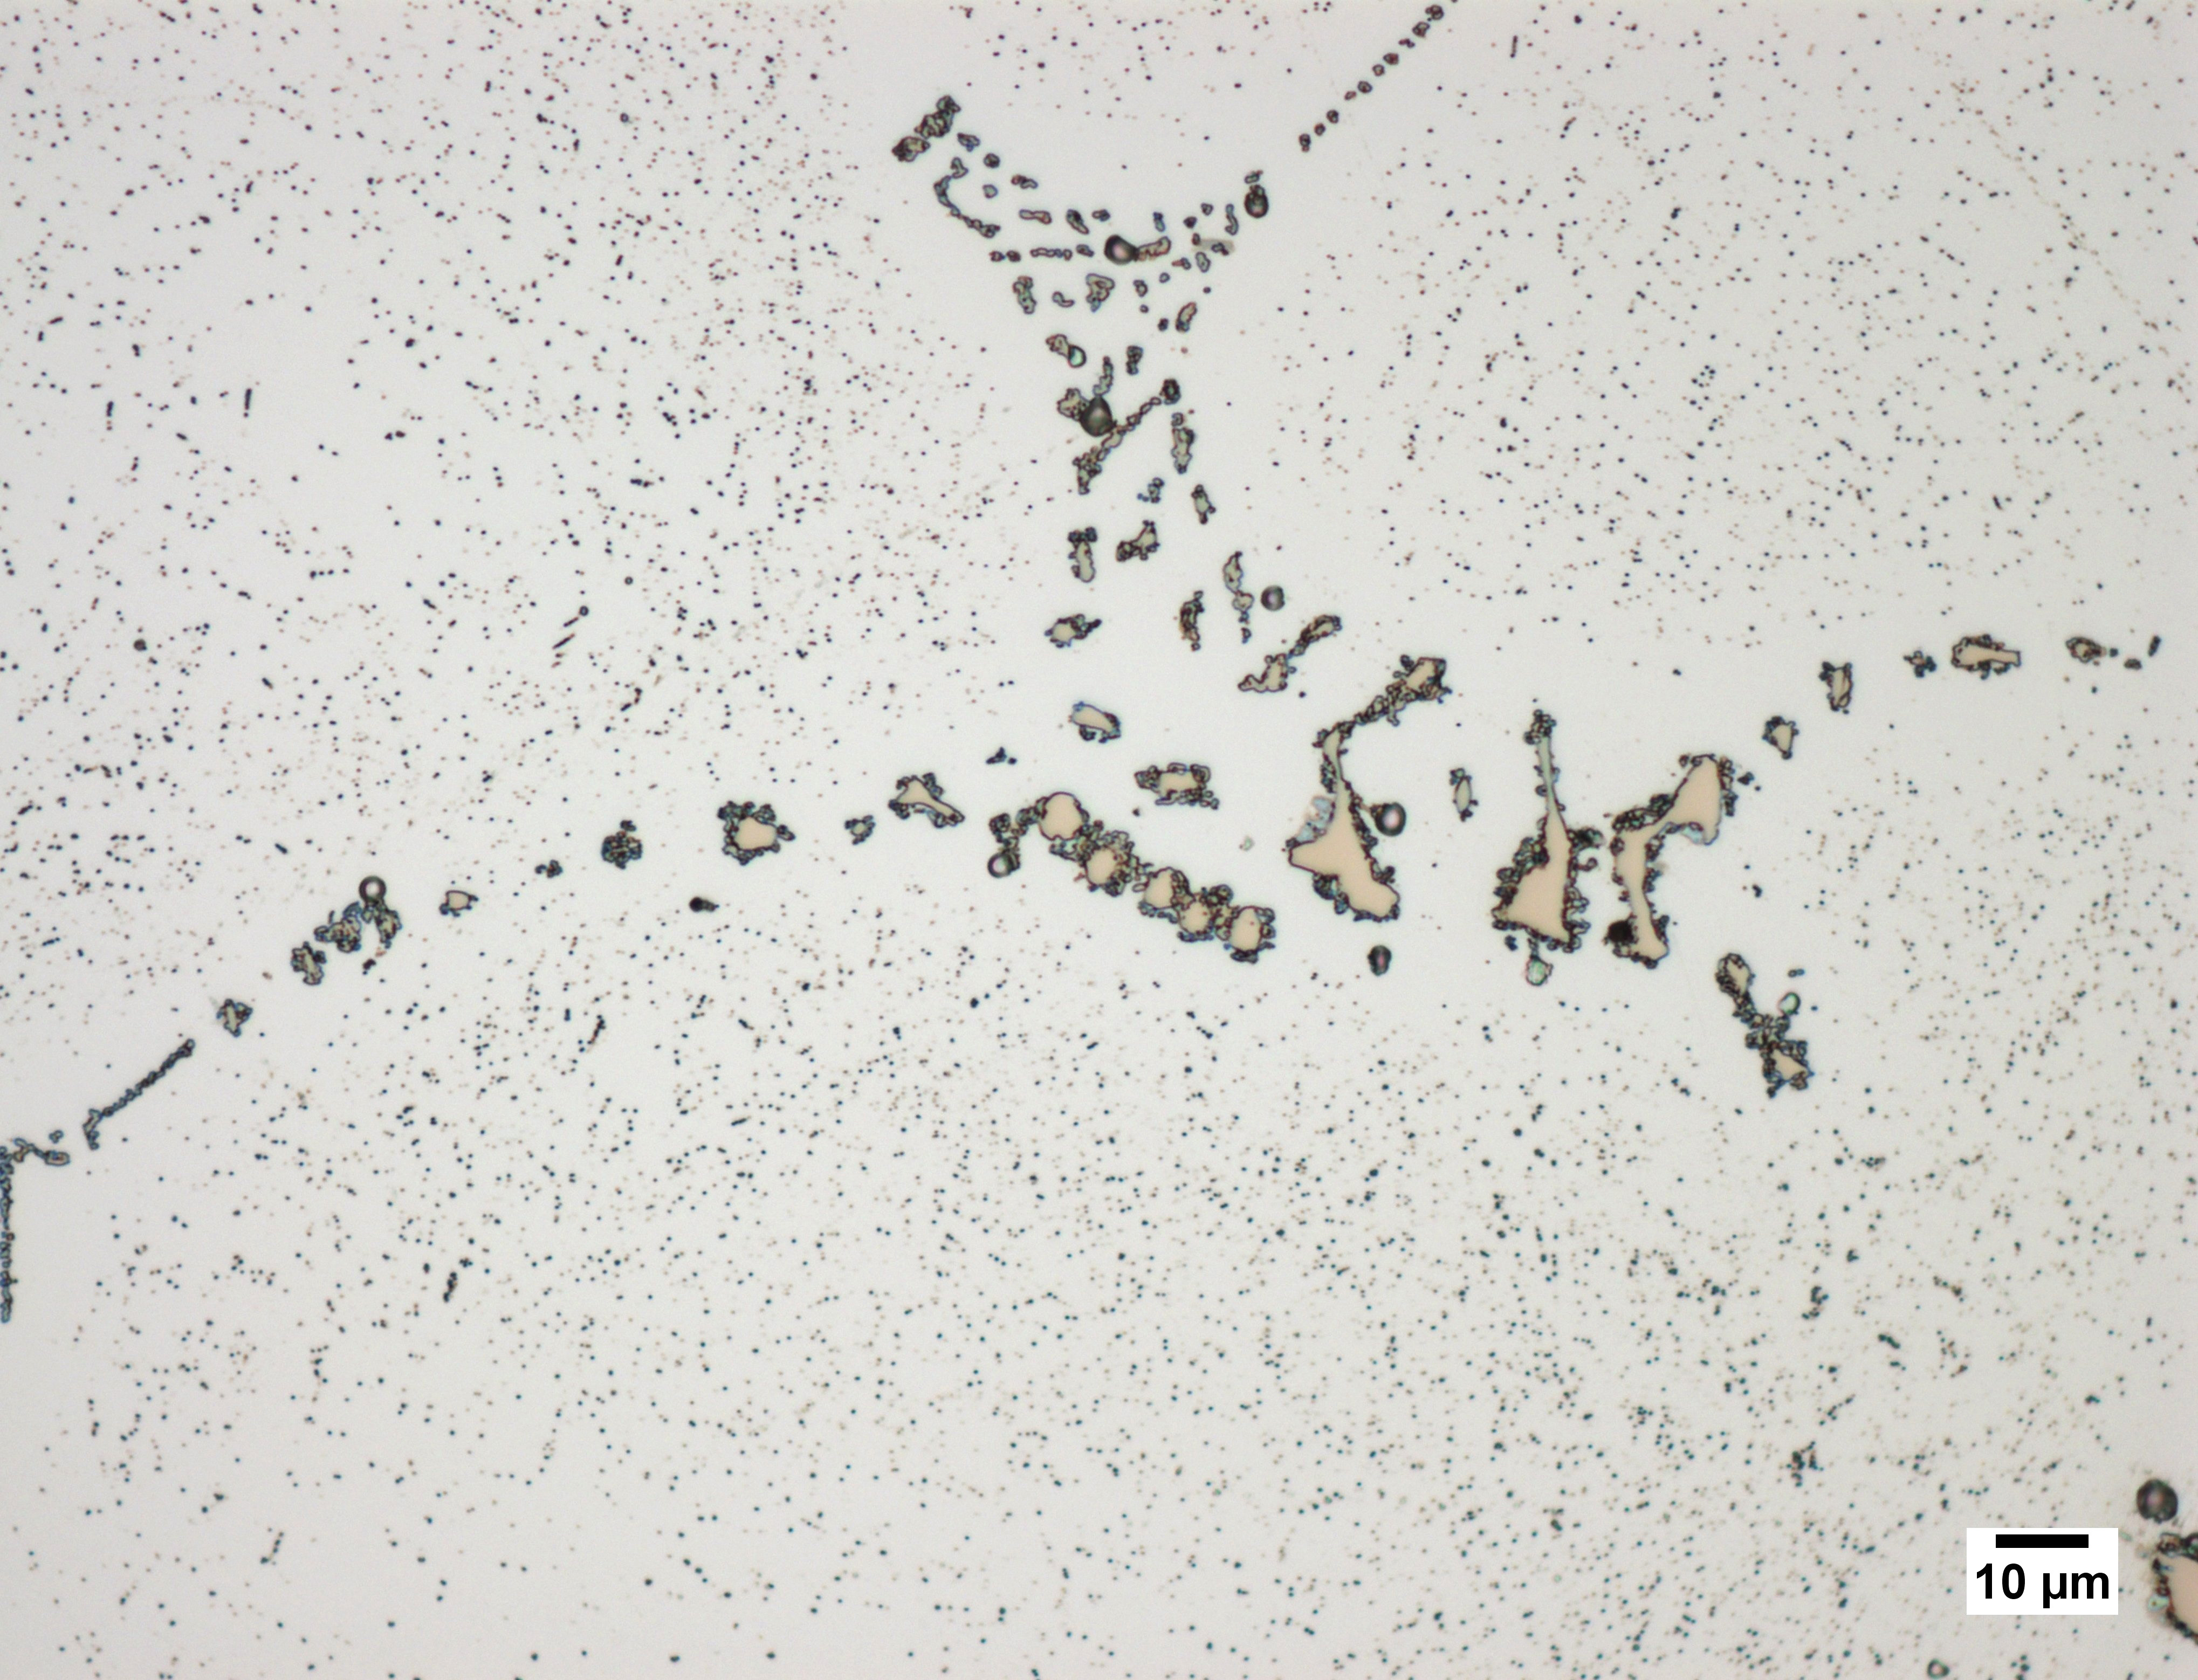
\includegraphics[width=4.7in]{figures/metallography/c5-oh-2375-remote-500x}}

% \caption{Optical Micrographs Showing the Microstructure of Unaffected Base Metal (Remote from the Fracture Location) in the Cone~5 2375\textdegree{}F On-Heating (\gls{zdt}) Hot Ductility Sample at (A) 200X and (B) 500X.  Etch: electrolytic 10\% oxalic acid.}
% \label{fig:c5-oh-2375-remote}
% \end{figure}



% Previous investigations (Hoffman and Colwell 1998; Hoffman and Gapinski 2001) of service-exposed 20Cr-32Ni-1Nb material with similar time in service indicated that the larger interdendritic phases were primarily niobium carbides (NbC), some of which were surrounded by a phase rich in Ni, Nb, and Si, while the intradendritic precipitates were determined to be mainly chromium carbides which precipitated as a result of service exposure.  The previously noted similarities in the hot ductility behavior are explained in light of the similarity of the as-received microstructures of the Cone~1 (``service-exposed'') and Cone~5 (``solution-annealed'') materials.  However, this was not the expected result based on the nominally reported material conditions since an earlier study on the repair weldability of 20Cr-32Ni-1Nb by Shi et al. (Shi, Lippold, and Ramirez 2010) indicated that solution annealed material showed a significantly different hot ductility response in terms of both on-heating and on-cooling behavior as compared to service-exposed material.  Therefore, the similar as-received microstructures of both Cone~1 and Cone~5, and the consequent similarities observed in the hot ductility characteristics, suggests that the weld joint region of Cone~5 (where the samples were extracted) was either not subjected to a solution annealing heat treatment or the parameters (temperature/time) were not adequate for an effective solution anneal, contrary to the information provided at the outset of this investigation.


% Regarding the Cone~5 On-Heating 2375\textdegree{}F (ZDT) hot ductility sample, examination of Figure 10a indicates that regions near the fracture surface showed a noticeably reduced extent of matrix precipitates compared a region remote from the fracture surface  (Figure 11).  This reduction is due to the dissolution of precipitates as a result of the high temperature exposure from the simulated thermal cycle.  It is also apparent from Figure 10a that the crack paths proceed along the interdendritic boundaries; Figure 10c and Figure 10d show that the crack faces appear to be associated with the interdendritic secondary phases.  Cracking proceeds along these boundaries because they are the regions corresponding to the greatest degree of solute segregation and resulting formation of low-melting point constituents; consequently, melting will begin at these regions first during the high temperatures imposed during the simulated thermal cycle of the hot ductility test.  The identity of the interdendritic phases has not yet been verified but this will be pursued as part of the future work.